\section{Procedure}

\soft{HALFpipe} starts up as a terminal-based user interface that prompts
the user with a series of questions about the dataset being analyzed and
the desired analysis plan. The main stages of \soft{HALFpipe} analysis,
which are detailed below, include loading data, preprocessing with
\soft{fMRIPrep}, quality assessment, feature extraction, and group-level
statistics. Users have the flexibility to specify the settings for each
processing stage at one time or separately at each stage. If
\soft{HALFpipe} is stopped and resumed at an intermediate stage,
\soft{HALFpipe} will detect which stages have been completed and ask the
user to indicate further analyses that are desired. For instance, the user
can request preprocessing and feature extraction, but not group-level
statistics, and later resume processing specifying group-level statistics
only.

\subsection{Loading data}

A major advantage of \soft{HALFpipe} is that it accepts input data
organized in various formats without the need for file naming conventions
or a specific directory structure. Using the terminal interface, the user
is asked to provide the location of the T1-weighted and fMRI BOLD image
files, which are required for preprocessing, as well as field maps and task
event files if available or applicable. However, \soft{HALFpipe} requires
additional information linking the image files to run in an automated
fashion, such as information specifying which set of images belong to the
same subject.

Through the use of path templates, \soft{HALFpipe} can handle a wide range
of folder structures and data layouts. The syntax for path templates is
adapted from \soft{C-PAC}'s data configuration \parencite{cpac_config}. Instead
of manually adding each input file for each subject separately, as is done
in the \soft{SPM} or \soft{FSL} user interfaces, the template describes the pattern used
for naming files. That pattern can match many file names, thereby reducing
the amount of manual work for the user. For example, when placing the tag
\filename{\{subject\}} in the file path \filename{\{subject\}\_t1.nii.gz},
all files of which the name ends in \filename{\_t1} and have the extension
\filename{.nii.gz} will be selected. The part of the filename that comes
before \filename{\_t1} is now interpreted by the parsing algorithm as the
subject identifier. When multiple files from different modalities have the
same subject identifier, or session number, etc., they will be matched
automatically by these tags. Automated processing workflows can then be
constructed around the resulting data structure. 

\begin{tablebox}[label={table:patterns}]{Examples of path template syntax}

\begingroup%
\fboxsep=1pt%
\newcolumntype{L}{>{\raggedright\arraybackslash}X}%
\newcolumntype{K}[1]{>{\raggedright\arraybackslash}m{#1}}%
\renewcommand{\arraystretch}{1.35}%
\begin{tabularx}{\textwidth}{@{} | K{2cm} |
L | L | @{}} 
\hhline{~|-|-|}
\multicolumn{1}{c|}{} & 
\textbf{Example 1} & 
\textbf{Example 2} \\
\hhline{-|-|-|}
Path template &%
\texttt{data/\colorbox{leaLightPurple}{\{subject\}}/bold\_rest.nii.gz} &%
\texttt{data/\colorbox{leaLightPurple}{\{subject\}}/bold\_\colorbox{leaLightBlue}{\{task\}}.nii.gz} \\
\hhline{-|-|-|}
Matches these files &%
\makecell[l]{%
\texttt{data/\colorbox{leaLightPurple}{subject01}/bold\_rest.nii.gz}\\%
\texttt{data/\colorbox{leaLightPurple}{subject02}/bold\_rest.nii.gz}\\%
\texttt{data/\colorbox{leaLightPurple}{subject03}/bold\_rest.nii.gz}\\%
\texttt{data/\colorbox{leaLightPurple}{phantom}/bold\_rest.nii.gz}} &%
\makecell[l]{%
\texttt{data/subject\colorbox{leaLightPurple}{01}/bold\_\colorbox{leaLightBlue}{rest}.nii.gz}\\%
\texttt{data/subject\colorbox{leaLightPurple}{02}/bold\_\colorbox{leaLightBlue}{rest}.nii.gz}\\%
\texttt{data/subject\colorbox{leaLightPurple}{03}/bold\_\colorbox{leaLightBlue}{rest}.nii.gz}\\%
\texttt{data/subject\colorbox{leaLightPurple}{01}/bold\_\colorbox{leaLightBlue}{task}.nii.gz}} \\
\hhline{-|-|-|}
Does not match &%
\makecell[l]{%
\texttt{data/subject01/bold\_\colorbox{leaLightGrey}{task}.nii.gz}\\%
\texttt{data/\colorbox{leaLightGrey}{subfolder}/subject01/bold\_rest.nii.gz}} &%
\makecell[l]{%
\texttt{data/\colorbox{leaLightGrey}{phantom}/bold\_rest.nii.gz}\\%
\texttt{data/\colorbox{leaLightGrey}{subfolder}/subject01/bold\_rest.nii.gz}} \\
\hhline{-|-|-|}
\end{tabularx}\par
\vspace*{2mm}
Note: The grey highlight shows the part of the file name that is
responsible for not matching.
\endgroup

\end{tablebox}


In contrast to \soft{C-PAC}'s data configuration syntax, \soft{HALFpipe}
path templates use BIDS tags \parencite{10.1038/sdata.2016.44}. \soft{HALFpipe}
path templates can be further specified by adding a colon and a regular
expression after the tag name (as in standard Python regular expression
syntax). For example, \filename{\{subject:[0-9]\*\}} will only match
subject identifiers that contain just digits. This can be useful for more
complex data layouts, such as when multiple datasets are placed in the same
directory, and only a single subset is to be used. For more examples, see
Table~\ref{table:patterns}.

In the \soft{HALFpipe} user interface, the user receives feedback on how
many and which files are matched, so that the path templates can be entered
interactively. Importantly, after finishing the configuration process via
the user interface, all files are internally converted into the
standardized BIDS structure, which is a prerequisite for running
\soft{fMRIPrep}. However, no copies of files are made, the conversion is
based entirely on symbolic links (aliases) to the original files. If the
data are already in BIDS format, \soft{HALFpipe} will still carry out this
conversion for consistency. The resulting dataset in BIDS format is then
stored in the working directory in a subfolder called \filename{rawdata}.

\subsection{Preprocessing}

Preprocessing is implemented in \soft{HALFpipe} using \soft{fMRIPrep},
which performs a consensus of preprocessing steps required for any fMRI
study \parencite{10.1038/s41592-018-0235-4}. The consensus steps include skull
stripping, tissue segmentation, and spatial normalization of structural
images. Consensus steps for functional images include motion correction,
slice time correction, susceptibility distortion correction, and spatial
normalization. Besides slice timing correction, all other steps entail
spatial transformations. \soft{fMRIPrep} calculates the parameters for each
of these transformations, which are combined and finally applied in one
step. The resulting image is outputted, among other derived data and a
report on preprocessing. Importantly, \soft{HALFpipe} runs \soft{fMRIPrep}
with small modifications. We disabled experimental susceptibility
distortion correction in the absence of field maps, because it is not yet
validated. We also do not output preprocessed and normalized functional
images by default, because they use a lot of disk space. However, users can
manually choose to output preprocessed images with their choice of
preprocessing settings in the user interface.

For fMRI data, \soft{HALFpipe} can perform denoising via \soft{ICA-AROMA}
\parencite{10.1016/j.neuroimage.2015.02.064}. Additional widely used
preprocessing steps, such as spatial smoothing, grand mean scaling,
temporal filtering (Gaussian- or frequency-based), and confound regression
can be selected by the user, the latter using confounds selected from the
large set generated by \soft{fMRIPrep}, including the original motion
parameters, derivatives of motion parameters, motion parameters squared,
top five aCompCor components \parencite{10.1016/j.neuroimage.2007.04.042},
white matter signal, CSF signal, and global signal. Importantly, in
\soft{fMRIPrep} all confound signals are extracted from the data before
\soft{ICA-AROMA} is run. If applicable, \soft{HALFpipe} will apply
denoising to these confound signals as well, to match the preprocessed and
denoised data, so as to not accidentally re-introduce noise variance
\parencite{10.1016/j.neuroimage.2013.05.116,10.1002/hbm.24528}. This was
illustrated with the example on motion parameter regression in the
section~\nameref{sec:denoising}.

Various confound and denoising settings may be used for each fMRI feature
(see section~\nameref{sec:featureextraction}), and for generating
preprocessed images that can, for example, be used to extract features with
software other than \soft{HALFpipe}.

\subsection{Quality assessment}

Quality assessment can be performed in an interactive, browser-based user
interface (see \autoref{fig:qa}). \soft{HALFpipe} provides a
detailed user manual for quality assessment that is linked on the web page.
The web app shows report images of several preprocessing steps such as T1
skull stripping and normalization, BOLD tSNR, motion confounds, ICA-based
artifact removal, and spatial normalization (see the methods section
on~\nameref{sec:qamethods}). These images can be visually inspected and
rated by the viewer as either good, uncertain, or bad.

Ratings will be saved in the local browser storage. Once completed, they
can be downloaded in JSON format to be read by \soft{HALFpipe}. If placed
in the working directory, ratings will be automatically detected by
\soft{HALFpipe} and used to exclude subjects for group-level statistics.
Additionally, \soft{HALFpipe} will automatically detect all other JSON
files whose names start with \filename{exclude}, to accommodate quality
assessment by multiple researchers. In the case of conflicts between
ratings, the lower rating will be used.

\soft{HALFpipe} will include as much data as possible while excluding all
scans rated as ``bad''. Ratings of ``good'' and ``uncertain'' will be
included for group analysis. A ``bad'' rating for any report image related
to structural/anatomical processing will exclude the entire subject. A 
``bad'' rating for any report image related to functional image processing
will only exclude the specific functional scan. This means that if a
subject has one ``bad'' scan, its other scans may still be included for
group statistics.

In addition, the mean framewise displacement, percentage of frames with a
framewise displacement above a specified threshold, percentage of the
independent components that were classified as noise, and mean gray matter
tSNR from all subjects is displayed in box plots. Next to the report
images, links to the source images are shown so that these can be inspected
in more detail by opening them in a preferred image viewer (e.g.,
\soft{fsleyes}).

\begin{figure}[!tb]
\begin{adjustwidth}{-1cm}{}
\hsize=\linewidth%
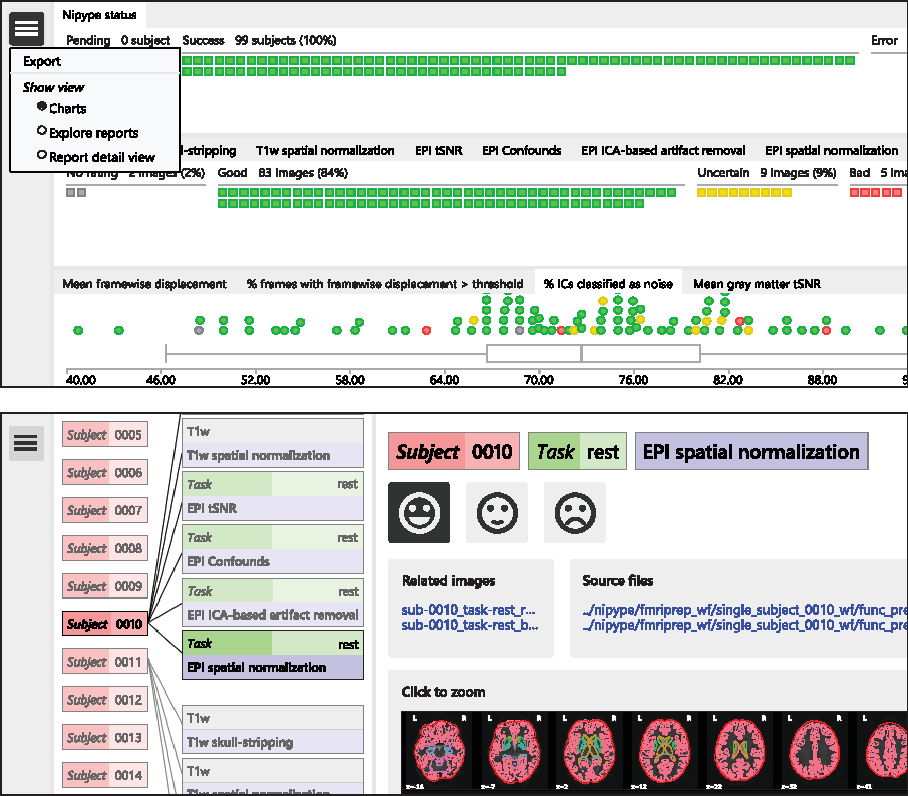
\includegraphics[width=\linewidth]{fig/quality_assessment-crop}
\caption{\textbf{Quality assessment user interface.} The top panel shows
the charts view, containing one chart for processing status, one for
quality ratings and one for image quality metrics. In the top left
corner, the navigation menu is open, which shows the option to export
ratings for use in group statistics. The bottom panel contains a 
screenshot of the explorer view that allows the user to navigate across
subjects and image types. The explorer view shows the currently selected
report image on the right, along with its rating, related images, and the
source files that were used to construct it.}\label{fig:qa}
\end{adjustwidth}
\end{figure}

\subsection{Feature extraction}\label{sec:featureextraction}

Following preprocessing, \soft{HALFpipe} can extract several
\term{features} that are commonly used in resting-state and task-based
analysis. These include various ways of examining functional connectivity
between brain regions (seed-based connectivity, network-template (or dual)
regression, atlas-based connectivity matrices), as well as measures of
local activity (ReHo, fALFF). \soft{HALFpipe} allows the user to choose
several region-of-interest masks (seeds), template networks, and atlases,
for which a threshold indicates the minimum overlap the user requires
between seeds, template networks, or atlas regions and the subjects' fMRI
data. For each feature, the user can change the default settings for
spatial smoothing and temporal filtering, and choose the confounds to be
removed. The user is offered the option to extract the same feature
multiple times, each time varying the preprocessing, confound, and
denoising settings to explore the impact of analytical decisions in a
\term{multiverse analysis}. Of note, for selected features some options are
not available. For example, spatial smoothing is disabled for atlas-based
connectivity matrices \parencite{10.1111/ejn.13717}, or performed \emph{after}
ReHo and fALFF have been calculated (see Table~\ref{table:settings}).

A brief description of the features is provided in Box~\ref{box:features}.

\subsection{Group-level statistics}

Group-level statistics on individual features can be performed with
\soft{FSL}'s FLAME algorithm. Subjects who had poor quality data in the
interactive quality assessment are excluded. In addition, subjects can be
excluded based on movement by selecting the maximum allowed mean framewise
displacement (FD) and percentage of outlier frames (i.e., frames with
motion higher than the specified FD threshold).

For group-level statistics, users can choose to calculate the intercept
only (i.e., mean across all subjects) or run flexible factorial models. For
the latter, \soft{HALFpipe} prompts the user to specify the path to a
covariates file (multiple file formats are supported) containing subject
identifiers, group membership, and other variables, and to specify whether
these are continuous or categorical. Missing values in the covariates file
can be handled with either listwise deletion or mean substitution. The user
can specify main effects and interactions between variables, while
within-group regressions against a continuous variable (e.g., symptom
severity) is also possible.

\begin{featurebox}[label={box:features}]{Overview of HALFpipe features}

\paragraph{Task-based activations}

A first-level general linear model (GLM) is run for event-related or block
designs. GLM regressors describing the stimulus presentations for each of
the task conditions are convolved with a double Gamma HRF and the overall
model is fit for each voxel in the brain using \soft{FSL FILM}
\parencite{woolrich_temporal_2001}. Contrasts of interest are tested, which
results in a whole-brain task activation map for comparisons between task
conditions.

\paragraph{Seed-based connectivity}

Average BOLD time series are extracted from a region of interest (seed),
which is defined by a binary mask image. This time series is used as a
regressor in a first-level GLM, where the model is fit for each voxel in
the brain using \soft{fsl\_glm}. This results in a whole-brain functional
connectivity map that represents the connectivity strength between the ROI
and each voxel in the brain.

\paragraph{Network-template (or dual) regression}

Subject-specific representations of connectivity networks (e.g., default
mode, salience, task-positive networks) are generated using dual regression
\parencite{beckmann_dual_reg_2009} with \soft{fsl\_glm}. In a first
regression model, the set of network template maps is regressed against the
individual fMRI data, which generates time series for each of the template
networks. Next, a second regression model is run, regressing the network
time series against the individual fMRI data. This generates
subject-specific spatial representations of each of the template networks,
which can be considered to represent the voxelwise connectivity strength
within each of the networks.

\paragraph{Atlas-based connectivity matrix}

Average time series are extracted from each region of a brain atlas of
choice using custom code inspired by \soft{Pypes}
\parencite{10.3389/fninf.2017.00025} and \soft{Nilearn}
\parencite{10.3389/fninf.2014.00014}. From these, a pairwise connectivity
matrix between atlas regions is calculated using Pearson product-moment
correlations using \soft{Pandas} \parencite{mckinney-proc-scipy-2010}, which
represent the pairwise functional connectivity between all pairs of regions
included in the atlas.

\paragraph{Regional homogeneity (ReHo)}

Local similarity (or synchronization) between the time series of a given
voxel and its nearest neighboring voxels is calculated using Kendall's
coefficient of concordance \parencite{10.1016/j.neuroimage.2003.12.030} using
\soft{FATCAT}'s \soft{3dReHo} which is distributed with \soft{AFNI}
\parencite{10.1089/brain.2013.0154}.

\paragraph{Fractional amplitude of low frequency fluctuations (fALFF)}

Variance in amplitude of low frequencies in the BOLD signal is calculated,
dividing the power in the low frequency range (0.01--0.1 Hz) by the power
in the entire frequency range \parencite{10.1016/j.jneumeth.2008.04.012} with a
customized version of the \soft{C-PAC} implementation of fALFF.\@

\end{featurebox}
